\documentclass{ximera}

\outcome{Identify an improper integral.}
\outcome{Determine if an improper integral converges or diverges.}
\outcome{Compute integrals over infinite intervals.}
\outcome{Compute integrals of functions with vertical asymptotes.}
\author{Jason Miller and Jim Talamo}
%\usepackage{todonotes}

\newcommand{\todo}{}

\usepackage{esint} % for \oiint
\ifxake%%https://math.meta.stackexchange.com/questions/9973/how-do-you-render-a-closed-surface-double-integral
\renewcommand{\oiint}{{\large\bigcirc}\kern-1.56em\iint}
\fi


\graphicspath{
  {./}
  {ximeraTutorial/}
  {basicPhilosophy/}
  {functionsOfSeveralVariables/}
  {normalVectors/}
  {lagrangeMultipliers/}
  {vectorFields/}
  {greensTheorem/}
  {shapeOfThingsToCome/}
  {dotProducts/}
  {partialDerivativesAndTheGradientVector/}
  {../productAndQuotientRules/exercises/}
  {../normalVectors/exercisesParametricPlots/}
  {../continuityOfFunctionsOfSeveralVariables/exercises/}
  {../partialDerivativesAndTheGradientVector/exercises/}
  {../directionalDerivativeAndChainRule/exercises/}
  {../commonCoordinates/exercisesCylindricalCoordinates/}
  {../commonCoordinates/exercisesSphericalCoordinates/}
  {../greensTheorem/exercisesCurlAndLineIntegrals/}
  {../greensTheorem/exercisesDivergenceAndLineIntegrals/}
  {../shapeOfThingsToCome/exercisesDivergenceTheorem/}
  {../greensTheorem/}
  {../shapeOfThingsToCome/}
  {../separableDifferentialEquations/exercises/}
}

\newcommand{\mooculus}{\textsf{\textbf{MOOC}\textnormal{\textsf{ULUS}}}}

\usepackage{tkz-euclide}\usepackage{tikz}
\usepackage{tikz-cd}
\usetikzlibrary{arrows}
\tikzset{>=stealth,commutative diagrams/.cd,
  arrow style=tikz,diagrams={>=stealth}} %% cool arrow head
\tikzset{shorten <>/.style={ shorten >=#1, shorten <=#1 } } %% allows shorter vectors

\usetikzlibrary{backgrounds} %% for boxes around graphs
\usetikzlibrary{shapes,positioning}  %% Clouds and stars
\usetikzlibrary{matrix} %% for matrix
\usepackage{pgfplots}
\usepgfplotslibrary{polar} %% for polar plots
\usepgfplotslibrary{fillbetween} %% to shade area between curves in TikZ
\usetkzobj{all}
\usepackage[makeroom]{cancel} %% for strike outs
%\usepackage{mathtools} %% for pretty underbrace % Breaks Ximera
%\usepackage{multicol}
\usepackage{pgffor} %% required for integral for loops



%% http://tex.stackexchange.com/questions/66490/drawing-a-tikz-arc-specifying-the-center
%% Draws beach ball
\tikzset{pics/carc/.style args={#1:#2:#3}{code={\draw[pic actions] (#1:#3) arc(#1:#2:#3);}}}



\usepackage{array}
\setlength{\extrarowheight}{+.1cm}
\newdimen\digitwidth
\settowidth\digitwidth{9}
\def\divrule#1#2{
\noalign{\moveright#1\digitwidth
\vbox{\hrule width#2\digitwidth}}}





\newcommand{\RR}{\mathbb R}
\newcommand{\R}{\mathbb R}
\newcommand{\N}{\mathbb N}
\newcommand{\Z}{\mathbb Z}

\newcommand{\sagemath}{\textsf{SageMath}}


%\renewcommand{\d}{\,d\!}
\renewcommand{\d}{\mathop{}\!d}
\newcommand{\dd}[2][]{\frac{\d #1}{\d #2}}
\newcommand{\pp}[2][]{\frac{\partial #1}{\partial #2}}
\renewcommand{\l}{\ell}
\newcommand{\ddx}{\frac{d}{\d x}}

\newcommand{\zeroOverZero}{\ensuremath{\boldsymbol{\tfrac{0}{0}}}}
\newcommand{\inftyOverInfty}{\ensuremath{\boldsymbol{\tfrac{\infty}{\infty}}}}
\newcommand{\zeroOverInfty}{\ensuremath{\boldsymbol{\tfrac{0}{\infty}}}}
\newcommand{\zeroTimesInfty}{\ensuremath{\small\boldsymbol{0\cdot \infty}}}
\newcommand{\inftyMinusInfty}{\ensuremath{\small\boldsymbol{\infty - \infty}}}
\newcommand{\oneToInfty}{\ensuremath{\boldsymbol{1^\infty}}}
\newcommand{\zeroToZero}{\ensuremath{\boldsymbol{0^0}}}
\newcommand{\inftyToZero}{\ensuremath{\boldsymbol{\infty^0}}}



\newcommand{\numOverZero}{\ensuremath{\boldsymbol{\tfrac{\#}{0}}}}
\newcommand{\dfn}{\textbf}
%\newcommand{\unit}{\,\mathrm}
\newcommand{\unit}{\mathop{}\!\mathrm}
\newcommand{\eval}[1]{\bigg[ #1 \bigg]}
\newcommand{\seq}[1]{\left( #1 \right)}
\renewcommand{\epsilon}{\varepsilon}
\renewcommand{\phi}{\varphi}


\renewcommand{\iff}{\Leftrightarrow}

\DeclareMathOperator{\arccot}{arccot}
\DeclareMathOperator{\arcsec}{arcsec}
\DeclareMathOperator{\arccsc}{arccsc}
\DeclareMathOperator{\si}{Si}
\DeclareMathOperator{\scal}{scal}
\DeclareMathOperator{\sign}{sign}


%% \newcommand{\tightoverset}[2]{% for arrow vec
%%   \mathop{#2}\limits^{\vbox to -.5ex{\kern-0.75ex\hbox{$#1$}\vss}}}
\newcommand{\arrowvec}[1]{{\overset{\rightharpoonup}{#1}}}
%\renewcommand{\vec}[1]{\arrowvec{\mathbf{#1}}}
\renewcommand{\vec}[1]{{\overset{\boldsymbol{\rightharpoonup}}{\mathbf{#1}}}}
\DeclareMathOperator{\proj}{\mathbf{proj}}
\newcommand{\veci}{{\boldsymbol{\hat{\imath}}}}
\newcommand{\vecj}{{\boldsymbol{\hat{\jmath}}}}
\newcommand{\veck}{{\boldsymbol{\hat{k}}}}
\newcommand{\vecl}{\vec{\boldsymbol{\l}}}
\newcommand{\uvec}[1]{\mathbf{\hat{#1}}}
\newcommand{\utan}{\mathbf{\hat{t}}}
\newcommand{\unormal}{\mathbf{\hat{n}}}
\newcommand{\ubinormal}{\mathbf{\hat{b}}}

\newcommand{\dotp}{\bullet}
\newcommand{\cross}{\boldsymbol\times}
\newcommand{\grad}{\boldsymbol\nabla}
\newcommand{\divergence}{\grad\dotp}
\newcommand{\curl}{\grad\cross}
%\DeclareMathOperator{\divergence}{divergence}
%\DeclareMathOperator{\curl}[1]{\grad\cross #1}
\newcommand{\lto}{\mathop{\longrightarrow\,}\limits}

\renewcommand{\bar}{\overline}

\colorlet{textColor}{black}
\colorlet{background}{white}
\colorlet{penColor}{blue!50!black} % Color of a curve in a plot
\colorlet{penColor2}{red!50!black}% Color of a curve in a plot
\colorlet{penColor3}{red!50!blue} % Color of a curve in a plot
\colorlet{penColor4}{green!50!black} % Color of a curve in a plot
\colorlet{penColor5}{orange!80!black} % Color of a curve in a plot
\colorlet{penColor6}{yellow!70!black} % Color of a curve in a plot
\colorlet{fill1}{penColor!20} % Color of fill in a plot
\colorlet{fill2}{penColor2!20} % Color of fill in a plot
\colorlet{fillp}{fill1} % Color of positive area
\colorlet{filln}{penColor2!20} % Color of negative area
\colorlet{fill3}{penColor3!20} % Fill
\colorlet{fill4}{penColor4!20} % Fill
\colorlet{fill5}{penColor5!20} % Fill
\colorlet{gridColor}{gray!50} % Color of grid in a plot

\newcommand{\surfaceColor}{violet}
\newcommand{\surfaceColorTwo}{redyellow}
\newcommand{\sliceColor}{greenyellow}




\pgfmathdeclarefunction{gauss}{2}{% gives gaussian
  \pgfmathparse{1/(#2*sqrt(2*pi))*exp(-((x-#1)^2)/(2*#2^2))}%
}


%%%%%%%%%%%%%
%% Vectors
%%%%%%%%%%%%%

%% Simple horiz vectors
\renewcommand{\vector}[1]{\left\langle #1\right\rangle}


%% %% Complex Horiz Vectors with angle brackets
%% \makeatletter
%% \renewcommand{\vector}[2][ , ]{\left\langle%
%%   \def\nextitem{\def\nextitem{#1}}%
%%   \@for \el:=#2\do{\nextitem\el}\right\rangle%
%% }
%% \makeatother

%% %% Vertical Vectors
%% \def\vector#1{\begin{bmatrix}\vecListA#1,,\end{bmatrix}}
%% \def\vecListA#1,{\if,#1,\else #1\cr \expandafter \vecListA \fi}

%%%%%%%%%%%%%
%% End of vectors
%%%%%%%%%%%%%

%\newcommand{\fullwidth}{}
%\newcommand{\normalwidth}{}



%% makes a snazzy t-chart for evaluating functions
%\newenvironment{tchart}{\rowcolors{2}{}{background!90!textColor}\array}{\endarray}

%%This is to help with formatting on future title pages.
\newenvironment{sectionOutcomes}{}{}



%% Flowchart stuff
%\tikzstyle{startstop} = [rectangle, rounded corners, minimum width=3cm, minimum height=1cm,text centered, draw=black]
%\tikzstyle{question} = [rectangle, minimum width=3cm, minimum height=1cm, text centered, draw=black]
%\tikzstyle{decision} = [trapezium, trapezium left angle=70, trapezium right angle=110, minimum width=3cm, minimum height=1cm, text centered, draw=black]
%\tikzstyle{question} = [rectangle, rounded corners, minimum width=3cm, minimum height=1cm,text centered, draw=black]
%\tikzstyle{process} = [rectangle, minimum width=3cm, minimum height=1cm, text centered, draw=black]
%\tikzstyle{decision} = [trapezium, trapezium left angle=70, trapezium right angle=110, minimum width=3cm, minimum height=1cm, text centered, draw=black]


\title[Dig-In:]{Improper Integrals}

\begin{document}
\begin{abstract}
  We can use limits to integrate functions on unbounded domains or functions with unbounded range.
\end{abstract}
\maketitle


Recall that we introduced the definite integral

\[
\int_a^b f(x) \d x,
\]

as a limit of Riemann sums.  This limit need not always exist, as it depended on the properties of the
function $f$ on the given interval $[a, b]$.  When the function $f$ is \emph{continuous} on $[a,b]$, this 
definite integral represented the net between the graph of $y=f(x)$ and the $x$-axis on $a \leq x \leq b$. 

\begin{image}
   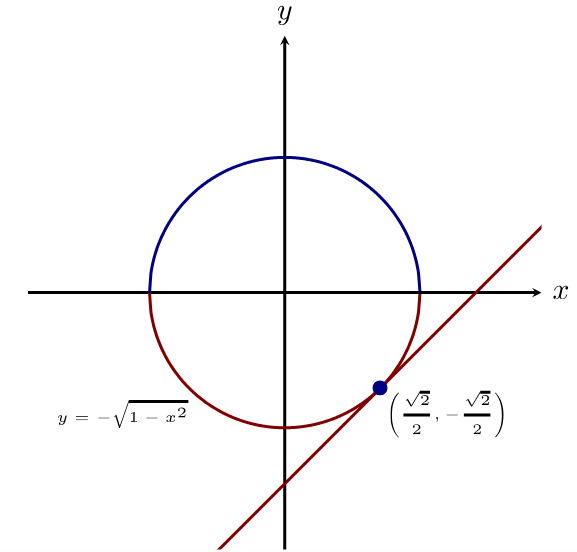
\includegraphics{1.png}
\end{image}


Actually computing the limit of Riemann sums is an arduous task, but in the case when $f$ is continuous on the finite interval $[a,b]$, the Fundamental Theorem of Calculus comes to the rescue and assures us that 

\begin{image}
   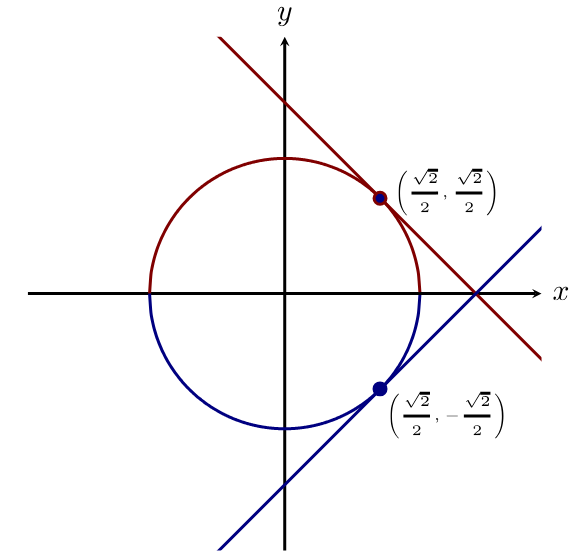
\includegraphics{2.png}
\end{image}

where $F(x)$ is an antiderivative of $f(x)$.

Note that in order to apply the Fundamental Theorem of Calculus, there are two requirements.

\begin{itemize}
\item The interval over which we integrated, $[a,b]$, must be a finite length
  interval, and
\item The function $f$ must be bounded on $[a,b]$.
\end{itemize}


\begin{remark}
Recall that in order for a function defined on $[a, b]$ to be bounded on $[a,b]$, there needs to exist an some real number $M>0$ such that 
\[
|f(x)| \leq M \text{ for all } x \text{ in } [a, b]
\]

This says that the outputs of $f$ are trapped between the horizontal lines $y=-M$ and $y=M$. Thus the output values cannot 
become arbitrarily large in either the positive or negative sense on $[a,b]$. 
\end{remark}


It turns out that there are many instances where these limitations are a problem.  For instance, there are applications in statistics, physics, and engineering where we need to integrate over unbounded regions or we need to integrate unbounded functions.  In this section, we will generalize the notion of the integral in such a way to overcome each of the restrictions above.



\begin{definition}
  An integral $\int_a^b f(x) \d x $
  is called an \dfn{improper integral} if one of, or both, of the conditions hold:
  \begin{itemize}
  \item The interval of integration is infinite.
  \item The function $f$ is unbounded on the interval of integration.
  \end{itemize}
\end{definition}

\begin{question}
  Which of the following integrals are improper according to the previous definition?
  \begin{selectAll}
    \choice{$\int_{-1}^{100} \frac{1}{1+x^2} \d x$}
    \choice[correct]{$\int_{1}^{\infty}\frac{1}{1+x^2}\d x$}
    \choice[correct]{$\int_0^1 \ln(x) \d x$}
    \choice{$\int_0^1 \frac{\sin(x)}{x} \d x$}
    \choice[correct]{$\int_{-\infty}^{\infty} \sin(x) \d x$}
    \choice[correct]{$\int_{0}^{\pi} \tan(x) \d x$}
  \end{selectAll}

\begin{feedback}
\begin{itemize}
\item Note that $\frac{1}{1+x^2}$ is continuous everywhere, so it is bounded on any finite interval. 
\item $\lim_{x \to 0^+} \ln(x) = -\infty$, so $\ln(x)$ is unbounded on $[0,1]$.
\item $\lim_{x \to 0^+} \frac{\sin(x)}{x} = 1$, so even though $\frac{\sin(x)}{x}$ is not continuous at $x=0$, it is bounded on $[0,1]$.  Hence $\int_0^1 \frac{\sin(x)}{x} \d x$ is proper.
\item $\tan(x)$ has a vertical asymptote at $x=\frac{\pi}{2}$, so it is unbounded on $[0,\pi]$.
\end{itemize}
\end{feedback}
\end{question}





\section{Unbounded intervals}


Consider the expression
\[ 
\int_{a}^{\infty} f(x) \d x
\]
What does this expression mean?  Let's consider a particular example and see if we can make sense of it.

\begin{example}
Evaluate the improper integral
\[ 
\int_{1}^{\infty} \frac{1}{x} \d x
\]
\begin{explanation}

We interpret definite integrals as giving us the net area underneath the graph of the function over the given interval. If we used this interpretation here, this notation should mean that we want to find the area under $\frac{1}{x}$ from $1$ to $\infty$.  This idea needs to be more precisely defined.  Let's consider the definite integral
\[
\int_{1}^{b} \frac{1}{x} \d x=\eval{\ln|x|}_{1}^{b}=\ln(b)
\]

where $b \geq 1$ is some fixed number. 

\begin{image}
   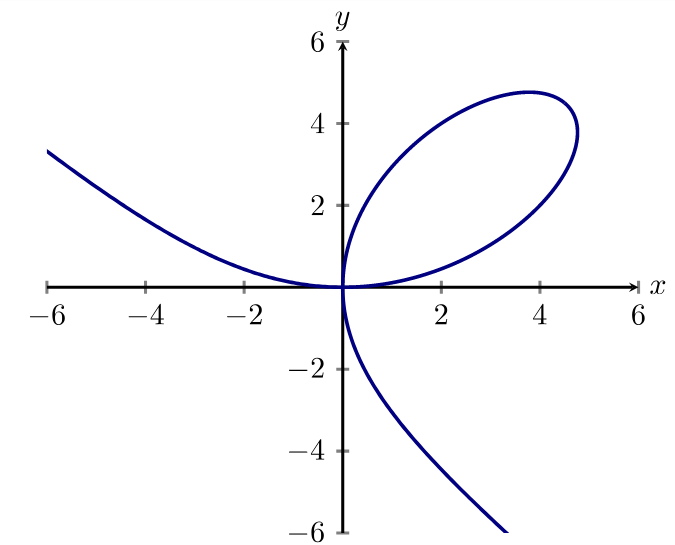
\includegraphics{3.png}
\end{image}


 This integral gives us the area underneath $1/x$ from $1$ to $b$. If we wanted to make sense of the integral to $\infty$, we could think of letting $b$ 
get larger and larger and seeing how this affects the area. 

That is, we interpret the integral from 1 to $\infty$ as a limit of a definite integral:

\[
\int_{1}^{\infty} \frac{1}{x} \d x= \lim_{b \to \infty} \int_{1}^{b} \frac{1}{x} \d x= \lim_{b \to \infty} \ln(b) = \infty
\]

We can interpret this result to mean that the area under $\frac{1}{x}$ from $1$ to $\infty$ is infinite.
\end{explanation}
\end{example}

It might seem like we should always get an answer of infinity or negative infinity if we integrate over an unbounded region, but the next example shows that is not always the case.

\begin{example}
Compute 
\[
\int_{1}^{\infty} \frac{1}{x^2} \d x
\]

\begin{explanation}
The previous example shows us we should consider this expression to be the limit of a definite integral 
in the following manner:

\[
\int_{1}^{\infty} \frac{1}{x^2} \d x=\lim_{b \to \infty} \int_{1}^{b} \frac{1}{x^2} \d x
\]

We calculate the definite integral 
\[
\int_{1}^{b} \frac{1}{x^2} \d x= \eval{\frac{-1}{x}}_{1}^{b}=1-\frac{1}{b}
\]

This gives the area under $\frac{1}{x^2}$ on the interval $[1, b]$. 

\begin{image}
   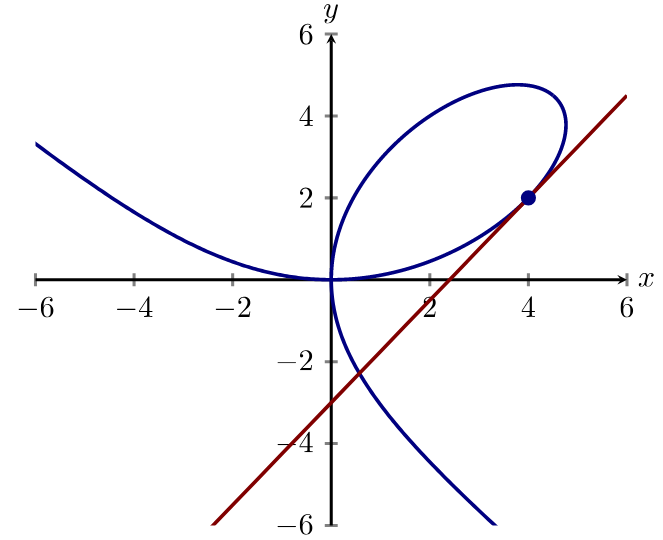
\includegraphics{4.png}
\end{image}

Now we take the limit of this area as $b \to \infty$. 

\[
\int_{1}^{b} \frac{1}{x^2} \d x= \lim_{b \to \infty} 1-\frac{1}{b}=1
\]
  
In this case, when we take the limit, we get a finite number, namely $1$. This suggests that we can consider the 
area under $1/x^2$ from $1$ to $\infty$ to be equal to $1$ despite the fact that the region is unbounded. 



\end{explanation}
\end{example}





%In the previous two examples we have seen we can assign a meaning to expressions like $\int_{a}^{\infty} f(x) \d x$
%by interpreting such an expression as shorthand for the following limit.

%\[
%\int_{a}^{\infty} f(x) \d x:=\lim_{N \to \infty} \int_{a}^{N} f(x) \d x
%\]
%
%We say that such integrals are \textbf{improper}. We will see other types of improper integrals later. 

%If the limit exists, that is, the limit is equal to a finite number $L$, then we say that the improper integral converges and we say the integral is equal to $L$. 
%If the limit does not exist, we say that the improper integral diverges. 


Thus in the two examples we have studied so far we have 


\[
\int_{1}^{\infty} \frac{1}{x} \d x = \infty
\]

\begin{image}
   \includegraphics{5.png}
\end{image}

and 

\[
\int_{1}^{\infty} \frac{1}{x^2} \d x =1
\]


\begin{image}
   \includegraphics{6.png}
\end{image}

Why do we get such different answer in these two cases?  The difference lies in the speed with which each function approaches $0$ as $x \to \infty$. Although both functions approach $0$ as $x \to \infty$, the function $\frac{1}{x^2}$ becomes smaller much more rapidly than $\frac{1}{x}$. 
We can see in the graphs above that $\frac{1}{x^2}$ shrinks down to zero much more quickly. The key idea is that the area that we are accumulating as $x\to \infty$ is shrinking rapidly enough that the total area stays bounded. This is a theme we will see again when we study convergence of series. 

We now give a precise definition for integrals over unbounded regions.

\begin{definition}\hfil
\begin{itemize}
\item Let $f$ be a continuous function on $[a,\infty)$.
  \[
  \int_a^\infty f(x) \d x \text{ is defined to be } \lim_{b\to\infty}\int_a^b f(x) \d x
  \]
\item Let $f$ be a continuous function on $(-\infty,b]$.
  \[
  \int_{-\infty}^b f(x) \d x \text{ is defined to be } \lim_{a\to-\infty}\int_a^b f(x) \d x
  \]
\item Let $f$ be a continuous function on $(-\infty,\infty)$. Let $c$
  be any real number.
  \[
  \int_{-\infty}^\infty f(x) \d x \text{ is defined to be }
  \]
  \[
  \lim_{a\to-\infty}\int_a^c f(x) \d x + \lim_{b\to\infty}\int_c^b
  f(x) \d x
  \]
\end{itemize}
An improper integral is said to \dfn{converge} if its corresponding
limit exists and is equal to a real number. Otherwise, the improper
integral is said to \dfn{diverge}. 
%In this case, the integral either does not exist, or is equal to $-\infty$ or $\infty$.
\end{definition}

\begin{warning}
  The improper integral $  \int_{-\infty}^\infty f(x) \d x$ converges if and only if \textbf{both}  $ \lim_{a\to-\infty}\int_a^c f(x) \d x$
and $  \lim_{b\to\infty}\int_c^b f(x) \d x$
independently converge.
\end{warning}

\begin{example}
Determine whether the integral
\[
\int_{-\infty}^{\infty} \frac{1}{1+x^2} \d x 
\]
converges or diverges. If it converges, determine the value of the integral. 
\begin{explanation}
Here both of the bounds of integration involve $\infty$ so to reinterpret the integral in terms of limits of definite integrals, 
we must first break up the integral into two pieces.

\begin{align*}
\int_{-\infty}^{\infty} \frac{1}{1+x^2} \d x&= \int_{-\infty}^{0} \frac{1}{1+x^2} \d x + \int_{0}^{\infty} \frac{1}{1+x^2} \d x \\
& =\lim_{a \to -\infty} \int_{a}^{0} \frac{1}{1+x^2} \d x + \lim_{b \to \infty} \int_{0}^{\infty} \frac{1}{1+x^2} \d x 
\end{align*}
 
Now we must look at each integral separately. 

\[
\int_{0}^{b} \frac{1}{1+x^2} \d x =  \answer{\arctan(b)}
\]


Similarly we obtain

\[
\int_{a}^{0} \frac{1}{1+x^2} \d x= \answer{-\arctan(a)}
\]
 
%\begin{hint}
%Recall that 
%  \[
%  \int \frac{1}{1+x^2} \d x = \arctan(x)+C,
%  \]
%  \end{hint}

Now we take the limits of each integral

\begin{question}
Determine the following limits:

 \begin{prompt}
   \[
    \lim_{b\to\infty} \arctan(b) = \answer{\pi/2}
    \]

\[
\lim_{M \to -\infty} -\arctan(M)=\answer{\pi/2}
\]
  \end{prompt}
\end{question}

Hence we have

\[
\int_{-\infty}^{\infty} \frac{1}{1+x^2} \d x=\lim_{M \to -\infty} \int_{M}^{0} \frac{1}{1+x^2} \d x + \lim_{b \to \infty} \int_{0}^{\infty} \frac{1}{1+x^2} \d x =\answer{ \pi}
\]
In this example, both integrals converge and therefore the entire integral converges. 
\end{explanation}
\end{example}







\begin{example}	
  Compute:
  \[
  \int_{-\infty}^{-1}\frac{-1}{x\sqrt{x^2-1}} \d x
  \]
  \begin{explanation}
    Write with me,
    \begin{align*}
      \int_{-\infty}^{-1} \frac{1}{x\sqrt{x^2-1}} \d x &= \lim_{a \to -\infty} \int_{a}^{-1} \frac{-1}{x\sqrt{x^2-1}}\d x\\
      &= \lim_{a \to -\infty} \eval{\answer[given]{\arcsec(x)}}_{a}^{-1} \\
      &= \lim_{a \to -\infty} \left(\arcsec(-1) - \arcsec(a)\right)\\
      &= \answer[given]{\pi - \frac{\pi}{2}}.
    \end{align*}
  \end{explanation}
  \end{example}

\begin{example}	
  Compute:
  \[
  \int_{-\infty}^\infty \sin(\theta) \d \theta
  \]
  \begin{explanation}
    Write with me:
    \[
    \int_{-\infty}^\infty \sin(\theta) \d \theta = \lim_{a\to -\infty} \int_a^1 \sin(\theta) \d \theta + \lim_{b\to\infty}\int_1^b \sin(\theta) \d \theta.
    \]
    Let us evaluate these limits one at a time:
    \begin{align*}  
      \lim_{a\to -\infty}\eval{-\cos(\theta)}_a^1 &= \lim_{a\to -\infty}\left(-\cos(1)+\cos(a)\right)\\
      &= \lim_{a\to -\infty} \cos(a) -\cos(1)\\
      &= \answer[given]{DNE}.
    \end{align*}
    We can stop here. Since one limit did not exist, the integral is
    divergent, and hence does not exist (DNE). We do not need to evaluate the other integral.
  \end{explanation}
\end{example}


\begin{warning}
In the last example, what would have happened if we had tried to
compute the indefinite integral with \textbf{a single limit}?
\[
\lim_{c\to \infty}\int_{-c}^c \sin(\theta)\d \theta?
\]
Since sine is an odd function on any bounded interval $[-c,c]$, we
would have found this integral to be $0$. However,
\[
\int_{-\infty}^\infty \sin(\theta) \d \theta \ne \lim_{c\to \infty}\int_{-c}^c \sin(\theta)\d \theta.
\]
We must compute \textbf{two limits} to correctly evaluate this
integral.
\end{warning}














%  &= \lim_{t\to 0^+} \left(\answer[given]{-1 -t \ln(t) +t}\right) \\
%    &= -1.


%Compare our last example to
%\[
%\int_{-\infty}^0 e^x \d x.
%\]
%This is equal to
%\begin{align*}
%  \int_{-\infty}^0 e^x \d x &= \lim_{a\to -\infty} \int_a^0 e^x \d x\\
%  &= \lim_{a\to-\infty}\eval{e^x}_{a}^0 \\
%  &= \lim_{a\to-\infty}\left(e^0 - e^a\right) \\
%  &=1.
%\end{align*}
%
%
%\begin{question}
%  Is it an accident that
%  \[
%  \int_{-\infty}^0 e^x \d x = \left| \int_0^1 \ln(x)\d x \right|?
%  \]
%  \begin{prompt}
%  \begin{multipleChoice}
%    \choice{yes}
%    \choice[correct]{no}
%  \end{multipleChoice}
%  \begin{feedback}
%    Since $\ln(x)$ is the inverse function of $e^x$, these integrals
%    are computing the same geometric area.
%  \end{feedback}
%  \end{prompt}
%\end{question}

%
%What is a practical example of an improper integral?  Sometimes in the
%real world it is useful to compute using infinity because we are
%interested in limiting behavior, or because we want to measure
%something which is ``effectively'' infinite in some way ( that is, really, really
%large).
%
%\begin{example}
%  How much work is required to move an $m\unit{kg}$ object from the
%  surface of the Earth out to a distance where the gravitation force
%  between the object and the Earth can be disregarded?
%
%  As a gesture of friendship, we will tell you the following facts:
%  The force of gravity between two objects of mass $M$ and $m$ in
%  kilograms at a distance of $x$ meters is given by
%  \[
%  F(x) = G\cdot \frac{m\cdot M}{x^2},
%  \]
%  where $G$ is the gravitational constant. 
%  \begin{explanation}
%    To start, we will work in terms of $m$, $M$, and $G$. In this
%    problem we are accumulating large forces over infinitesimal
%    distances. Hence
%    \begin{align*}
%      \d W &= F \d x\\
%      &= \answer[given]{G\cdot \frac{m\cdot M}{x^2}} \d x
%    \end{align*}
%    We can approximate ``really, really far away'' with ``infinitely
%    far away''. Write with me,
%    \begin{align*}
%      \mathrm{Work} &= \int_1^\infty F \d x\\
%      &= \int_1^\infty G\frac{m\cdot M}{x^2} \d x\\
%      &= G\cdot m\cdot M \lim_{\answer[given]{b} \to \infty} \eval{\answer[given]{-\frac{1}{x}}}_1^b\\
%      &=G\cdot m\cdot M \lim_{b \to \infty} \left(\answer[given]{1 - \frac{1}{b}}\right)\\
%      &=\answer[given]{G\cdot m\cdot M}.
%    \end{align*}
%  \end{explanation}
%\end{example}

\end{document}
